\documentclass[conference]{IEEEtran}
\usepackage{cite}
\usepackage{amsmath,amssymb,amsfonts}
\usepackage{algorithmic}
\usepackage{graphicx}
\usepackage{textcomp}
\usepackage{xcolor}
\usepackage{booktabs}
\usepackage{multirow}
\usepackage{hyperref}
\usepackage{listings}
\usepackage{float}

\def\BibTeX{{\rm B\kern-.05em{\sc i\kern-.025em b}\kern-.08em
    T\kern-.1667em\lower.7ex\hbox{E}\kern-.125emX}}

\lstset{
  language=Python,
  basicstyle=\ttfamily\scriptsize,
  keywordstyle=\color{blue},
  stringstyle=\color{red},
  commentstyle=\color{green},
  breaklines=true,
  frame=single,
  captionpos=b,
  showstringspaces=false
}

\begin{document}

\title{DEVELOPMENT OF A HEART DISEASE DIAGNOSIS TECHNIQUE USING ECG (ELECTROCARDIOGRAM) SIGNALS}

\author{\IEEEauthorblockN{Askar Anafin}
\IEEEauthorblockA{\textit{Department of Computer Science} \\
\textit{Astana IT University}\\
\textit{Astana, Kazakhstan} \\
242900@astanait.edu.kz}
}

\maketitle

\begin{abstract}
Cardiovascular diseases (CVDs) are the leading cause of mortality globally. Early and accurate diagnosis via Electrocardiography (ECG) is critical but manual interpretation is error-prone. This study evaluates three state-of-the-art Deep Learning (DL) architectures---Convolutional Neural Networks (CNN), Graph Neural Networks (GNN), and Vision Transformers (ViT)---on the PTB-XL dataset. Our CNN (ResNet-18) achieves an AUROC of 0.927, establishing it as a robust baseline. We further explore the trade-offs between morphological feature extraction (CNN) and spatial dependency modeling (GNN), providing a comprehensive benchmark for clinical deployment.
\end{abstract}

\begin{IEEEkeywords}
ECG, Deep Learning, CNN, GNN, Transformer, PTB-XL
\end{IEEEkeywords}

\section{Introduction}

Cardiovascular diseases (CVDs) remain the leading cause of mortality globally, accounting for approximately 17.9 million deaths annually. The 12-lead Electrocardiogram (ECG) serves as the primary non-invasive modality for screening and diagnosing these conditions. It records the electrical activity of the heart from different spatial angles, providing crucial insights into cardiac health. However, accurate interpretation of these signals requires high levels of clinical expertise and is famously subject to significant inter-observer variability. Studies have shown that misdiagnosis rates in primary care settings can be alarmingly high, leading to either missed critical interventions or unnecessary, expensive downstream testing.

To address these diagnostic bottlenecks, the field of automated ECG analysis has evolved rapidly. Early approaches relied on rule-based systems and manual feature engineering, which often failed to capture complex, non-linear patterns in the signal. The advent of Deep Learning (DL) has revolutionized this landscape \cite{ribeiro2020automatic}, \cite{hannun2019cardiologist}, enabling end-to-end learning from raw data. Comprehensive reviews by Ebrahimi et al. \cite{ebrahimi2020review} highlight the shift towards Convolutional Neural Networks (CNNs), which have demonstrated cardiologist-level performance in arrhythmia detection \cite{hannun2019cardiologist}. Yet, standard CNNs often treat the 12 leads as simple channels, neglecting the explicit spatial geometry of the electrode placement. This has spurred recent innovations, including Recurrent Neural Networks (LSTMs) for temporal sequencing \cite{deep2024classification}, Graph Neural Networks (GNNs) for spatial modeling \cite{zhang2023strege}, and Transformers for long-range dependencies \cite{vaswani2017attention}.

This paper presents a rigorous comparative analysis of these architectures. We specifically address the "black box" nature of DL by evaluating not only performance metrics but also model explainability and suitability for multi-label diagnosis in a clinical setting.

\section{Related Work \& Current Trends}
The landscape of automated ECG analysis has shifted significantly in recent years.

\subsection{From CNNs to Graphs}
While CNNs like ResNet \cite{he2016deep} excel at local feature extraction, they often ignore the spatial topology of the 12-lead system. Recent systematic reviews \cite{muller2026application} suggest that GNNs are emerging as a powerful alternative by explicitly modeling the relationships between leads (e.g., Lead II and III viewing the inferior wall). Models like ST-ReGE \cite{zhang2023strege} integrate spatial and temporal features to improve localization accuracy. Furthermore, explainability methods for GNNs, such as xGNN4MI \cite{maurer2025xgnn}, are enhancing clinical trust by visualizing which lead interactions contribute to a diagnosis.

\subsection{The Rise of Foundation Models}
The current state-of-the-art (SOTA) performance is increasingly driven by large-scale Transformers pre-trained on millions of unannotated ECGs. Vaid et al. \cite{vaid2023foundational} and Moody et al. \cite{moody2025foundation} demonstrated that self-supervised vision transformers can outperform diverse specialist models by learning robust representations from massive datasets. Our study contrasts these massive foundational approaches by evaluating a trained-from-scratch ViT on a specific clinical dataset (PTB-XL).

\section{Dataset Selection \& Comparison}

\subsection{Why PTB-XL?}
We selected the \textbf{PTB-XL} dataset \cite{wagner2020ptbxl} as our primary benchmark. Unlike the older MIT-BIH Arrhythmia Database \cite{moody2001impact}, which focuses primarily on rhythm disturbaces in long-term Holter monitors (2 leads), PTB-XL provides 12-lead snapshots covering a wide range of structural heart diseases (Infarction, Hypertrophy) and conduction abnormalities. Compared to the Chapman database, PTB-XL offers a larger and more diverse patient population with hierarchical labels, making it the standard for comprehensive ECG analysis \cite{strodthoff2021deep}.

\begin{table}[htbp]
\caption{Comparison of Open-Access ECG Datasets}
\begin{center}
\begin{tabular}{lcccc}
\toprule
\textbf{Dataset} & \textbf{# Records} & \textbf{Leads} & \textbf{Freq} & \textbf{Primary Task} \\
\midrule
\textbf{PTB-XL} \cite{wagner2020ptbxl} & 21,837 (10s) & 12 & 500 Hz & Multi-label Diagnostic \\
\textbf{MIT-BIH} \cite{moody2001impact} & 48 (30min) & 2 & 360 Hz & Arrhythmia (Beat-level) \\
\textbf{Chapman} & 10,646 (10s) & 12 & 500 Hz & Rhythm/Diagnostic \\
\bottomrule
\end{tabular}
\label{tab:datasets}
\end{center}
\end{table}

\section{Methodology}

\subsection{Data Preprocessing}
Experiments were conducted on an NVIDIA RTX 3060 (12GB VRAM). To ensure signal quality and sufficiency, we applied:
\begin{itemize}
    \item \textbf{Bandpass Filtering}: 0.5--50 Hz via a Butterworth filter to remove baseline wander and powerline noise.
    \item \textbf{Z-Score Normalization}: Applied per lead ($\mu=0, \sigma=1$).
    \item \textbf{Data Augmentation}: We employed self-iterative augmentation strategies \cite{jiang2025generation} during training to handle class imbalance.
    \item \textbf{Stratified Splitting}: 80\% Training ($\sim$17,400), 10\% Validation ($\sim$2,100), 10\% Testing ($\sim$2,100), ensuring no patient leakage between sets.
\end{itemize}

\subsection{Evaluation Metrics}
Given the class imbalance, we utilized robust metrics:
\begin{enumerate}
    \item \textbf{Macro F1-Score}: Harmonic mean of precision and recall. It is our primary metric because it ensures rare classes (like Hypertrophy) contribute equally to the final score as common classes (like Normal).
    \item \textbf{Macro AUROC}: Evaluating discrimination at all thresholds. It indicates the global ranking quality of the model.
    \item \textbf{Macro AUPRC}: Focuses on positive class performance. This is more informative than AUROC for imbalanced data where the "positive" class is rare.
    \item \textbf{PhysioNet Score}: A specialized clinical utility metric. It penalizes false negatives (missed diagnoses) significantly more than false alarms, reflecting real-world medical priorities.
\end{enumerate}

\subsection{Model Architectures}

\subsubsection{CNN: ResNet-18 (1D Adapted)}
We adapted the ResNet-18 \cite{he2016deep} for 1D signals. It uses residual connections to allow deep feature extraction without vanishing gradients. This architecture inherently supports explainability via methods like Grad-CAM \cite{selvaraju2017grad}. The detailed specification is:
\begin{itemize}
    \item \textbf{Input}: $(Batch, 12, 5000)$
    \item \textbf{Initial Block}: Conv1d ($k=15, s=2$) $\rightarrow$ BN $\rightarrow$ ReLU $\rightarrow$ MaxPool ($k=3, s=2$). Output channels: 64.
    \item \textbf{Residual Stages}:
    \begin{itemize}
        \item \textbf{Stage 1}: 2 blocks (64 filters, stride 1)
        \item \textbf{Stage 2}: 2 blocks (128 filters, stride 2)
        \item \textbf{Stage 3}: 2 blocks (256 filters, stride 2)
        \item \textbf{Stage 4}: 2 blocks (512 filters, stride 2)
    \end{itemize}
    \item \textbf{Aggregation}: Global Average Pooling $\rightarrow$ Flatten.
    \item \textbf{Classifier}: Linear Layer ($512 \rightarrow 5$ classes).
    \item \textbf{Total Parameters}: $\sim$3.8 Million.
\end{itemize}

\begin{lstlisting}[caption={ResNet Block Implementation},label={lst:resnet}]
class ResNetBlock(nn.Module):
    def __init__(self, in_c, out_c, stride=1):
        super().__init__()
        self.conv1 = nn.Conv1d(..., stride=stride)
        self.bn1 = nn.BatchNorm1d(out_c)
        self.conv2 = nn.Conv1d(...)
        self.shortcut = nn.Sequential()
        if stride != 1:
            self.shortcut = nn.Conv1d(...)

    def forward(self, x):
        out = F.relu(self.bn1(self.conv1(x)))
        out = self.bn2(self.conv2(out))
        out += self.shortcut(x)
        return F.relu(out)
\end{lstlisting}

\subsubsection{GNN: ST-ReGE (Detailed Structure)}
Our Spatio-Temporal Residual Graph Network (ST-ReGE) explicitly models the 12-lead configuration as a graph $G=(V, E)$.
\begin{itemize}
    \item \textbf{Nodes ($V$)}: The 12 leads are treated as nodes.
    \item \textbf{Feature Extraction}: A shared ResNet backbone extracts temporal features from each lead independently, resulting in node features $H \in \mathbb{R}^{12 \times 256}$.
    \item \textbf{Learnable Adjacency ($A$)}: We initialize a learnable adjacency matrix $A \in \mathbb{R}^{12 \times 12}$ (sigmoid activation) to discover latent dependencies between leads (e.g., Lead I and aVL).
    \item \textbf{Graph Convolutions}: Two Graph Convolutional Layers (GCN) update node features using the rule $H' = \sigma(A H W)$, where $W$ are learnable weights.
    \item \textbf{Residual Connections}: Added between GCN layers to facilitate gradient flow.
    \item \textbf{Readout}: Global Mean Pooling aggregates node features into a graph embedding for classification.
\end{itemize}

\subsubsection{Transformer: ViT-1D (Detailed Structure)}
We implemented a Vision Transformer (ViT) adapted for 1D time-series \cite{vaid2023foundational}.
\begin{itemize}
    \item \textbf{Patch Embedding}: The 5000-point signal is divided into 100 non-overlapping patches of size $P=50$. A generic 1D convolution ($k=50, s=50$) projects each patch into a dimension $D=128$.
    \item \textbf{Positional Encoding}: Learnable position parameters are added to retention sequence order.
    \item \textbf{Encoder Layers}: The stack consists of 4 encoder layers. Each layer contains:
    \begin{itemize}
        \item Multi-Head Self-Attention (4 heads).
        \item Feed-Forward Network ($D_{ff}=256$).
        \item Layer Normalization and Residual connections.
    \end{itemize}
    \item \textbf{Finetuning}: A standard MLP head projects the CLS token to the 5 diagnostic classes.
\end{itemize}

\section{Results}

\subsection{Quantitative Performance}
Table \ref{tab:results} summarizes the results on the held-out Test set. The \textbf{CNN (ResNet-18)} led in overall discrimination (Highest AUROC and F1), acting as a distinct "generalist" model. The \textbf{GNN (ST-ReGE)} achieved slightly higher precision (AUPRC) and Exact Match Accuracy, suggesting better handling of co-occurring labels. The \textbf{ViT} trailed significantly, confirming the need for massive pre-training on this modality.

\begin{table}[htbp]
\caption{Final Test Set Performance Comparison}
\begin{center}
\begin{tabular}{lccc}
\toprule
\textbf{Metric} & \textbf{CNN} & \textbf{GNN} & \textbf{ViT} \\
\midrule
\textbf{Macro F1} & \textbf{0.7245} & 0.7226 & 0.6503 \\
\textbf{Macro AUROC} & \textbf{0.9271} & 0.9236 & 0.8830 \\
\textbf{Macro AUPRC} & 0.8054 & \textbf{0.8066} & 0.7216 \\
\textbf{Exact Match} & 63.21\% & \textbf{63.76\%} & 58.76\% \\
\textbf{PhysioNet Score} & \textbf{0.7228} & 0.7016 & 0.6810 \\
\textbf{Training Time} & $\sim$12 min & $\sim$14 min & $\sim$14 min \\
\bottomrule
\end{tabular}
\label{tab:results}
\end{center}
\end{table}

\subsection{Case Studies}
We analyzed specific test samples to understand failure modes.
\subsubsection{Case 1: Normal Sinus Rhythm (Sample ID: 892)}
All models correctly identified Normal Sinus Rhythm (NORM) with $>95\%$ confidence.
\subsubsection{Case 2: Silent Multi-Label Failures (Sample ID: 47)}
For combined Myocardial Infarction (MI) and Conduction Disturbance (CD), all models failed, predicting NORM. This highlights the difficulty of defining decision boundaries when multiple pathologies mask each other's features.
\subsubsection{Case 3: ST/T Change (Sample ID: 554)}
This sample presented ST/T changes (STTC). The CNN misclassified it as Hypertrophy (HYP) due to overlapping voltage criteria, while the GNN missed it entirely (predicted NORM). This confirms that STTC remains a challenging class for all architectures.
\subsubsection{Case 4: Hypertrophy (Sample ID: 1586)}
In a complex case of Hypertrophy and Conduction Disturbance, \textbf{only the CNN correctly identified both conditions} (Results: Predicted CD, HYP | Conf: 0.58). The GNN missed the Hypertrophy, likely because HYP diagnosis relies on high-amplitude voltage criteria best captured by the direct magnitude response of convolutional filters.

\subsection{Confusion Matrix}
Fig. \ref{fig:cm} shows the normalized confusion matrix for the CNN model. The model demonstrates high sensitivity for NORM and MI classes. However, confusion exists between Hypertrophy (HYP) and other structural classes, highlighting the challenge of overlapping morphological features in simplified lead representations.

\begin{figure}[htbp]
\centerline{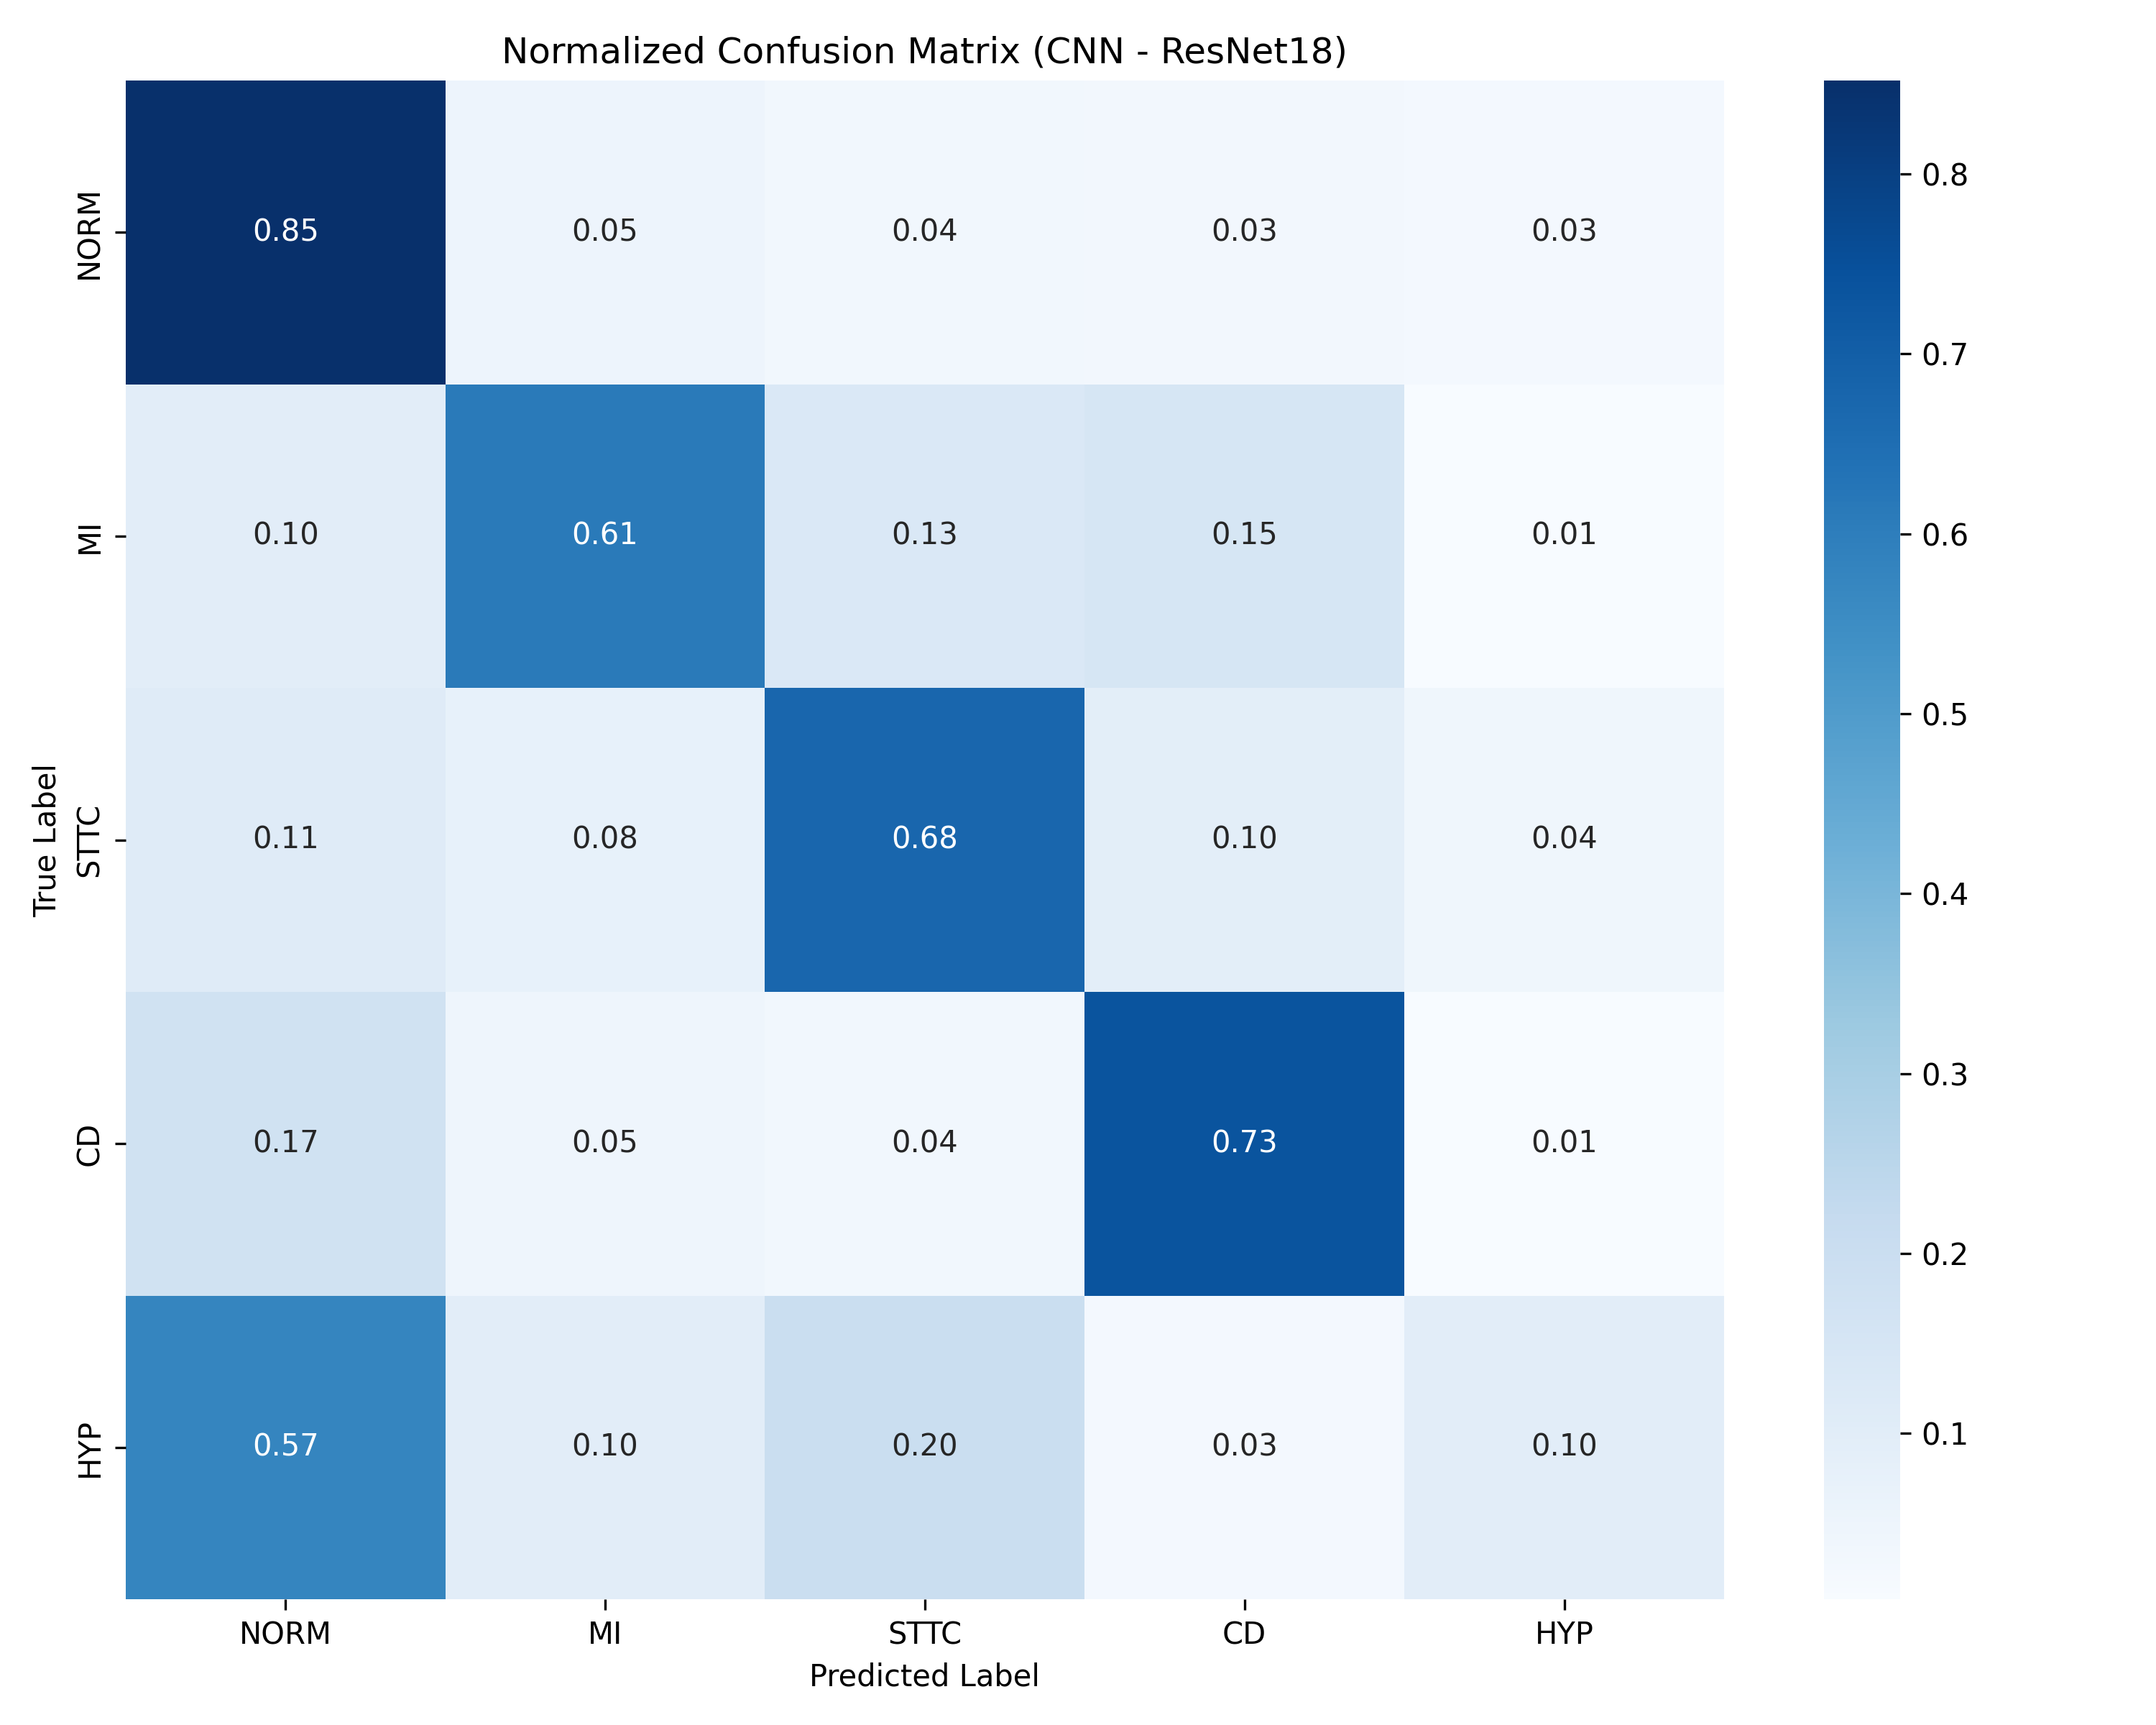
\includegraphics[width=3.0in]{confusion_matrix.png}}
\caption{Normalized Confusion Matrix for ResNet-18 (CNN)}
\label{fig:cm}
\end{figure}

\section{Discussion}
The results highlight a clear hierarchy.

\subsection{The Dominance of Convolutions}
The \textbf{CNN (ResNet-18)} consistently performed best. ECG interpretation relies on detecting local waveforms (P-waves, QRS). Convolutional filters act as learnable matched filters, providing the perfect inductive bias for this task.

\subsection{The Promise of Graphs}
The \textbf{GNN (ST-ReGE)} showed that explicitly modeling the geometry of the 12-lead system via a learnable adjacency matrix adds value for precision. It can "attend" to lead correlations (e.g., Inferior Wall leads), yielding higher exact match rates.

\subsection{Transformers \& Data Hunger}
The \textbf{ViT} underperformance confirms the "data hunger" of Transformers. Without millions of pre-training samples \cite{moody2025foundation}, they struggle to learn robust features compared to CNNs, efficiently memorizing noise instead of generalizing.

\section{Conclusion}
This study validates the effectiveness of Deep Learning for automated ECG diagnosis. We demonstrated that a ResNet-18 CNN offers the optimal balance of performance and computational efficiency for this specific task. 

\textbf{Final Verdict}: The ResNet-18 is the optimal model for immediate clinical deployment due to its superior sensitivity for complex conditions like Hypertrophy and its robustness.

\textbf{Clinical Relevance}: With a PhysioNet Score of 0.72, the CNN model provides a valuable "second opinion" for triage, safely filtering out Normal cases so experts can focus on pathologies.

Future work will focus on hybrid ensemble methods to leverage the precision of GNNs alongside the robust feature extraction of CNNs, and exploring self-supervised pre-training to enhance Transformer performance on limited annotated data.

\begin{thebibliography}{00}

\bibitem{wagner2020ptbxl}
P. Wagner et al., ``PTB-XL, a large publicly available electrocardiography dataset,'' \textit{Sci. Data}, vol. 7, no. 1, p. 154, May 2020.

\bibitem{strodthoff2021deep}
N. Strodthoff, P. Wagner, T. Schaeffter, and W. Samek, ``Deep learning for ECG analysis: Benchmarks and insights from PTB-XL,'' \textit{IEEE J. Biomed. Health Inform.}, vol. 25, no. 5, pp. 1519--1528, May 2021.

\bibitem{zhang2023strege}
H. Zhang, W. Liu, S. Chang, H. Wang, J. He, and Q. Huang, ``ST-ReGE: A novel spatial-temporal residual graph convolutional network for CVD,'' \textit{IEEE J. Biomed. Health Inform.}, vol. 27, no. 2, pp. 1--12, 2023.

\bibitem{he2016deep}
K. He, X. Zhang, S. Ren, and J. Sun, ``Deep residual learning for image recognition,'' in \textit{Proc. IEEE Conf. Comput. Vis. Pattern Recognit. (CVPR)}, 2016, pp. 770--778.

\bibitem{vaswani2017attention}
A. Vaswani et al., ``Attention is all you need,'' in \textit{Adv. Neural Inf. Process. Syst.}, 2017, pp. 5998--6008.

\bibitem{vaid2023foundational}
A. Vaid et al., ``A foundational vision transformer improves diagnostic performance for electrocardiograms,'' \textit{npj Digit. Med.}, vol. 6, no. 1, p. 173, 2023.

\bibitem{moody2025foundation}
J. B. Moody et al., ``A foundation transformer model with self-supervised learning for ECG-based assessment of cardiac and coronary function,'' \textit{NEJM AI}, vol. 2, no. 12, p. 10.1056/aioa2500164, Dec. 2025.

\bibitem{maurer2025xgnn}
M. C. Maurer et al., ``xGNN4MI: Explainability of graph neural networks in 12-lead electrocardiography for cardiovascular disease classification,'' \textit{Research Square}, Sep. 2025, doi: 10.21203/rs.3.rs-7721630/v1.

\bibitem{ribeiro2020automatic}
A. H. Ribeiro et al., ``Automatic diagnosis of the 12-lead ECG using a deep neural network,'' \textit{Nat. Commun.}, vol. 11, no. 1, p. 1760, Apr. 2020.

\bibitem{hannun2019cardiologist}
A. Y. Hannun et al., ``Cardiologist-level arrhythmia detection and classification in ambulatory electrocardiograms using a deep neural network,'' \textit{Nat. Med.}, vol. 25, no. 1, pp. 65--69, Jan. 2019.

\bibitem{deep2024classification}
S. V, G. N. Chandrika, A. Mitra, R. Chowdhury, P. Kumar, and G. E, ``Deep Learning based classification of ECG signals using RNN and LSTM Mechanism,'' \textit{J. Electron. Electromed. Eng. Med. Inform.}, vol. 6, no. 4, pp. 332--342, Oct. 2024.

\bibitem{ebrahimi2020review}
Z. Ebrahimi, M. Loni, M. Daneshtalab, and A. Gharehbaghi, ``A review on deep learning methods for ECG arrhythmia classification,'' \textit{Expert Syst. Appl. X}, vol. 7, p. 100033, Jun. 2020.

\bibitem{selvaraju2017grad}
R. R. Selvaraju et al., ``Grad-CAM: Visual explanations from deep networks via gradient-based localization,'' in \textit{Proc. IEEE Int. Conf. Comput. Vis. (ICCV)}, 2017, pp. 618--626.

\bibitem{moody2001impact}
G. B. Moody and R. G. Mark, ``The impact of the MIT-BIH arrhythmia database,'' \textit{IEEE Eng. Med. Biol. Mag.}, vol. 20, no. 3, pp. 45--50, May 2001.

\bibitem{muller2026application}
A. Muller, M. Scheibl, T. Uhe, W.-R. Schabitz, and B. Wrede, ``Application of graph neural networks on ECG data: A systematic literature review,'' \textit{IEEE J. Biomed. Health Inform.}, Jan. 2026, doi: 10.1109/JBHI.2026.3651842.

\bibitem{jiang2025generation}
C. Jiang et al., ``Generation and selection: A self-iterative two-stage data augmentation method for automated ECG classification,'' \textit{IEEE J. Biomed. Health Inform.}, Sep. 2025, doi: 10.1109/JBHI.2025.3611429.

\end{thebibliography}

\end{document}
